\documentclass{standalone}
\usepackage[T1]{fontenc}
\usepackage[utf8]{inputenc}
\usepackage{pgf,tikz}
\usepackage{pgfplots}
\pgfplotsset{compat=1.9}

\begin{document}

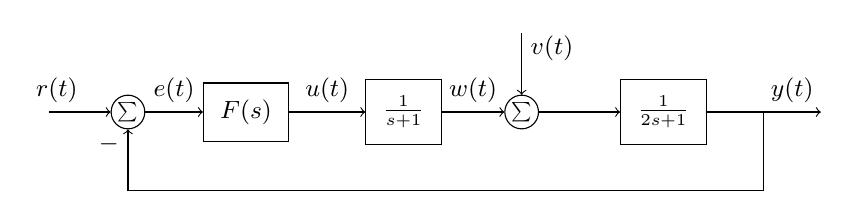
\begin{tikzpicture}
  {\small 
  \node[coordinate] (input) {};
  \node[circle, draw, right of=input, inner sep=1pt, scale=0.7] (sum) {$\sum$};
  \node[rectangle, draw, right of=sum, inner sep=6pt, node distance=1.5cm] (reg) {$F(s)$};
  \node[rectangle, draw, right of=reg, inner sep=6pt, node distance=2cm] (pump) {$\frac{1}{s+1}$};
  \node[circle, draw, right of=pump, inner sep=1pt, scale=0.7, node distance=1.5cm] (sum2) {$\sum$};
  \node[rectangle, draw, right of=sum2, inner sep=6pt, node distance=1.8cm] (tank) {$\frac{1}{2s+1}$};
  \node[coordinate, right of=tank, node distance=2cm] (output) {};
  \node[coordinate, below of=tank] (feedback) {};
  \node[coordinate, above of=sum2] (disturb) {};
 
  \draw[->] (tank) -- node[coordinate, inner sep=0pt] (meas) {} node[near end, above] {$y(t)$} (output);
  \draw[->] (meas) |- (feedback) -| node[very near end, left] {$-$} (sum);
  \draw[->] (input) -- node[very near start, above] {$r(t)$} (sum);
  \draw[->] (sum) -- node[above] {$e(t)$} (reg);
  \draw[->] (pump) -- node[above] {$w(t)$} (sum2);
  \draw[->] (sum2) -- (tank);
  \draw[->] (disturb) -- node[near start, right] {$v(t)$} (sum2);
  \draw[->] (reg) -- node[above] {$u(t)$} (pump);
}
\end{tikzpicture}
\end{document}
